\begin{frame}{Qu'est-ce une revue?}
  Devinez si les noms \alert{en gras} sont au masculin ou au féminin.\\
  \vspace{0.5cm}
  Une revue est un genre théâtral qui associe musique, danse et sketches qui font \underline{\uncover<2->{la}} \alert{satire} de personnes contemporaines, de l'\alert{actualité} (\uncover<3->{f.}) ou \underline{\uncover<4->{de la}} \alert{littérature}.
  Comme les \alert{formes} (\uncover<5->{f.}) apparentées de l'\alert{opérette} (\uncover<6->{f.}) et \underline{\uncover<7->{de la}} \alert{comédie} musicale, la revue allie musique, danse et comédie pour former \underline{\uncover<8->{un}} \alert{spectacle} complet.
  \underline{\uncover<9->{Un}} \alert{thème} général est utilisé pour \underline{\uncover<10->{un}} \alert{enchaînement} de numéros au cours desquels solos et ensembles de danse se relaient.
  
  \vspace{0.25cm}
  \begin{columns}
    \column{0.5\textwidth}
      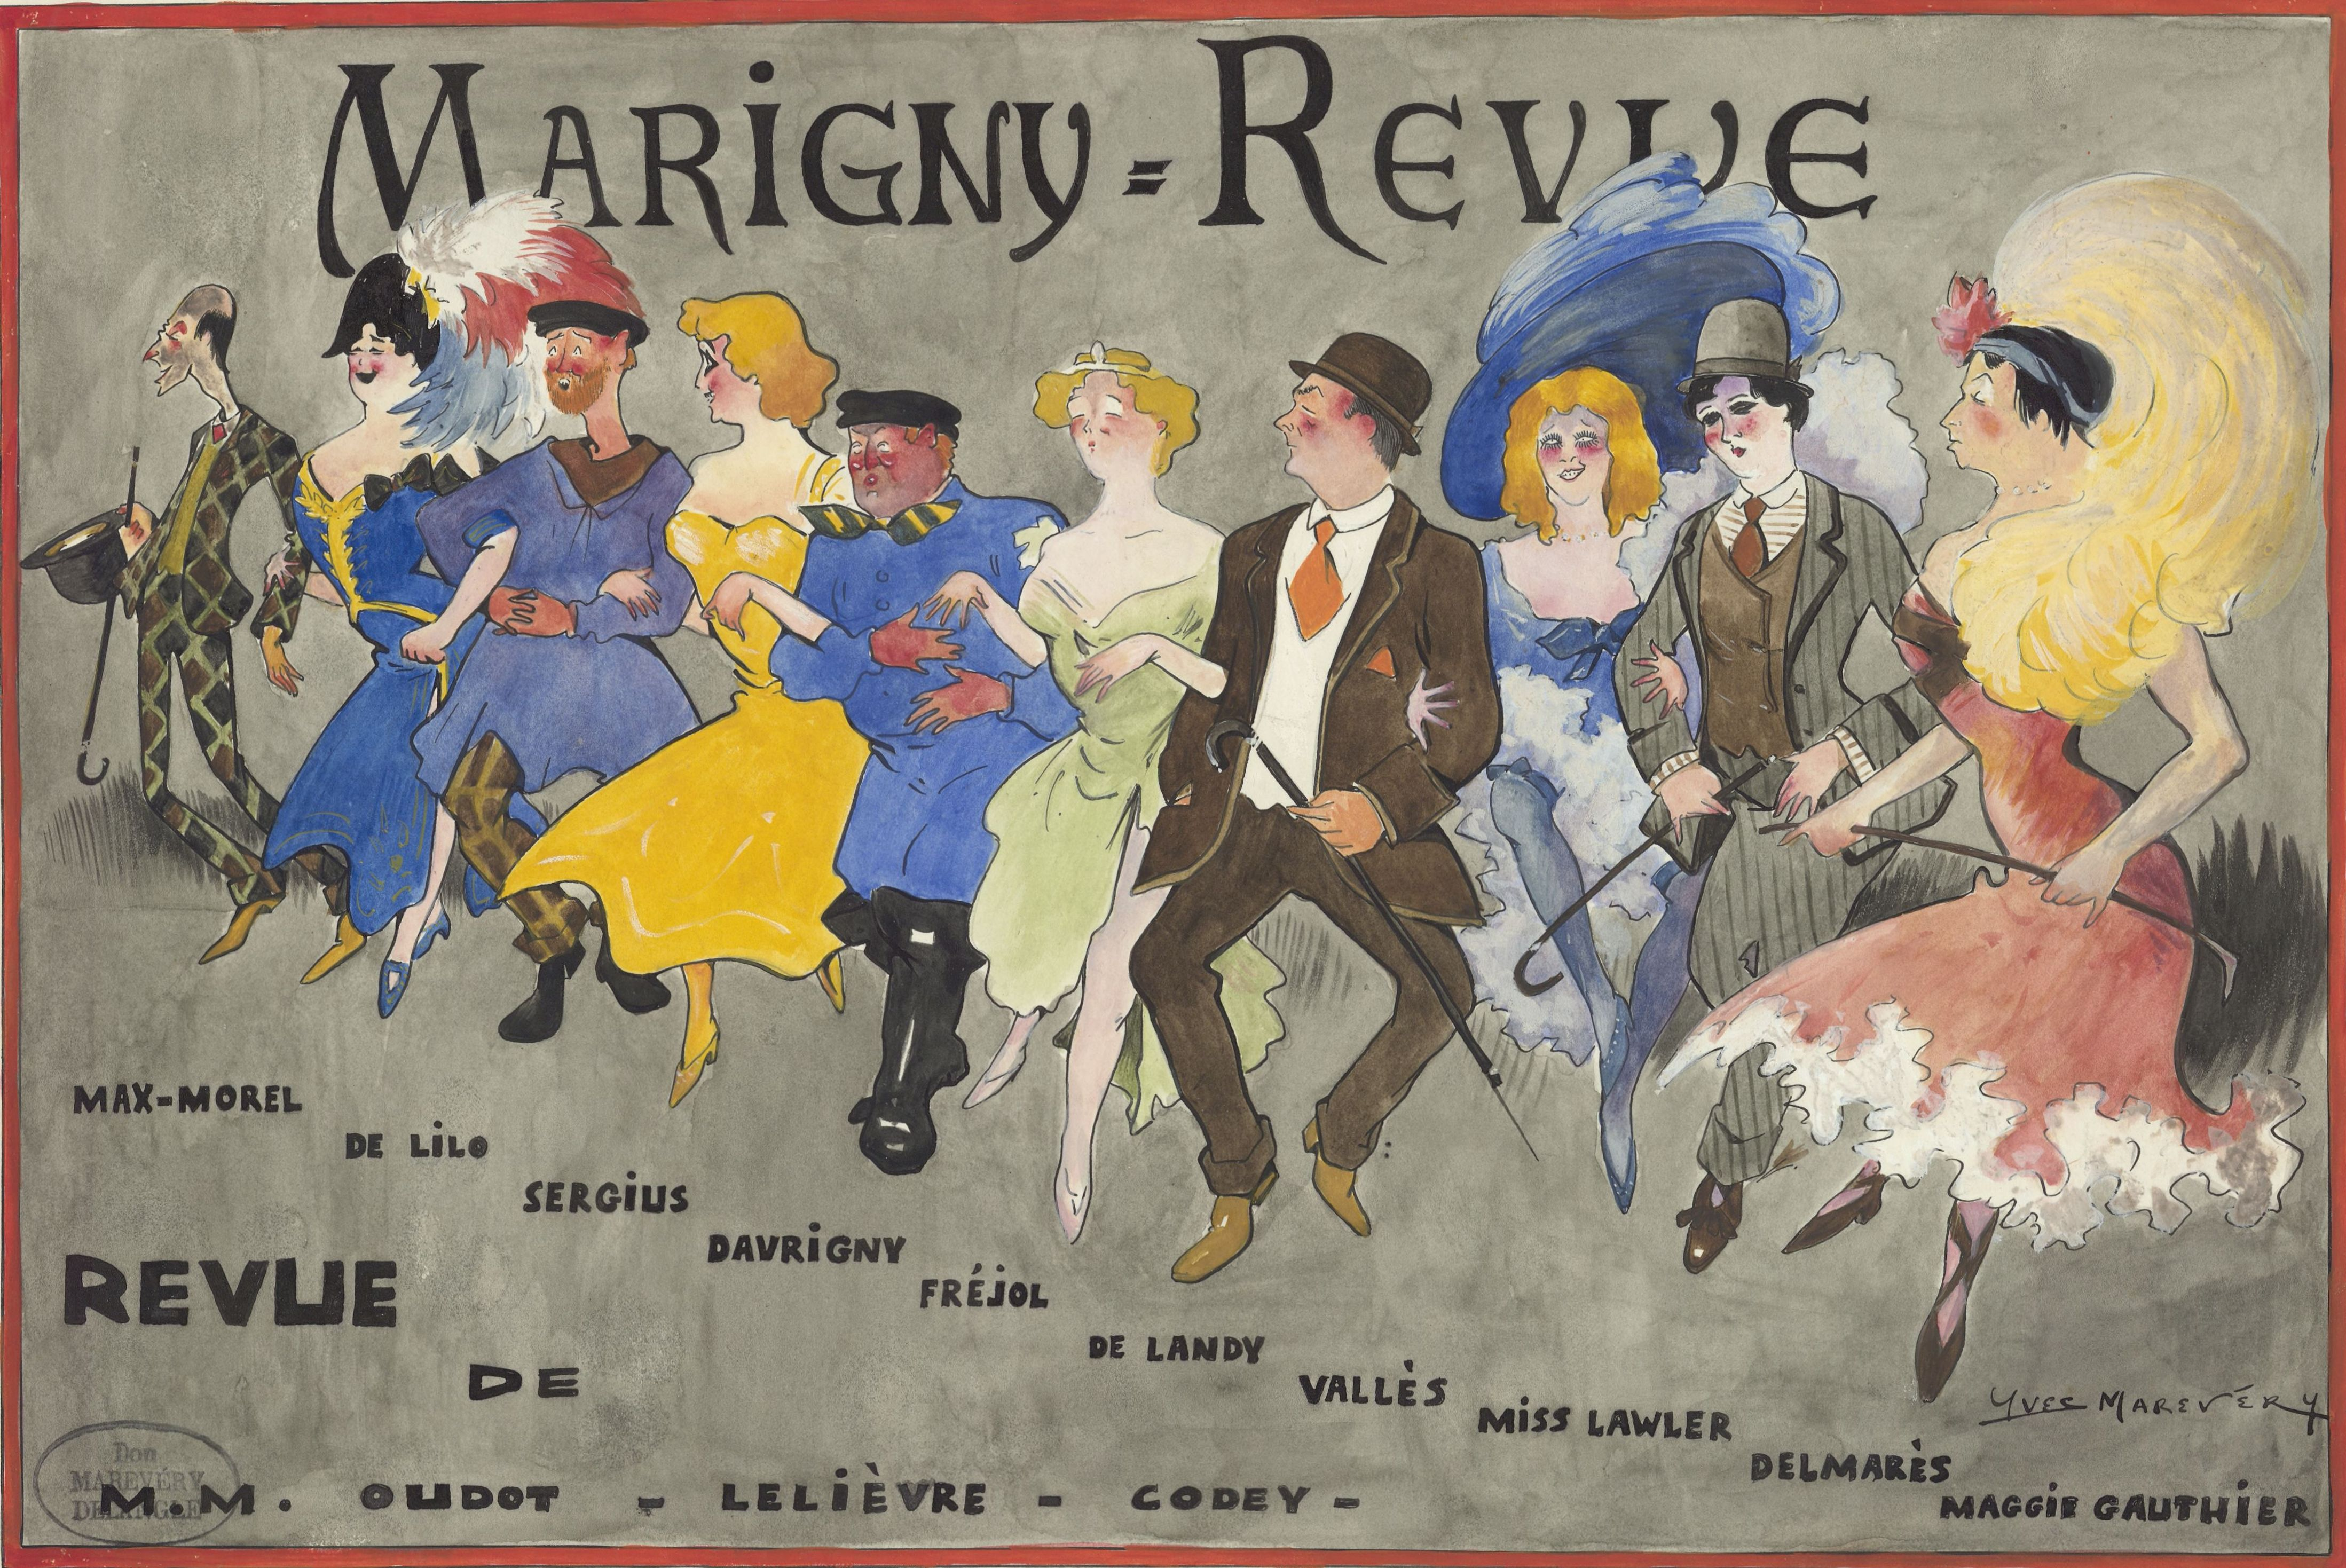
\includegraphics[scale=0.1]{revue.jpg}
    \column{0.5\textwidth}
      \raggedleft
      \hyperlink{début}{Au début}...
  \end{columns}
\end{frame}